\chapter{数据表示、探索与准备}
\label{chap:data}
\chaptergoal{能够读懂一张样本表，说明每列的含义与用途；使用Pandas读取、选择和检查数据；解释缺失值、类别编码和标准化；区分从训练数据确定处理规则与把规则应用到新数据。}

上一章已经认识了花的尺寸与物种记录。本章把“读懂数据”落实为可以执行的操作。重点不是记忆许多命令，而是让每一步都有明确对象：读入什么、改变什么、保留什么，以及处理后的表是否仍然对应原来的样本。

本章使用两个已经分工明确的例子：鸢尾花数据用于练习表格与散点图；接下来介绍的葡萄酒化学分析数据用于观察多种测量量的尺度。先理解记录的含义，再学习读取函数。

\section{从科学记录到样本表}
\subsection{数据表不只是一个数字矩阵}
\textbf{样本表}把记录按行排列，把字段按列排列。字段是有名称的一项记录内容，可以是测量值、类别、编号或质量说明。\textbf{字段字典}则是解释字段的附表，至少说明名称、含义、单位、数据类型和本次任务中的用途。它相当于实验记录本中对各列的说明，不能由程序自动猜出。

\textbf{CSV}是“逗号分隔值”（comma-separated values）的缩写，是一种用文本保存表格的文件形式。通常第一行写列名，后续每行写一条记录，相邻数值以逗号分隔。例如一份人为构造的长度测量表可以写为：
\begin{lstlisting}[language={},caption={用于理解CSV格式的人工三行示例，长度单位为厘米}]
record_id,length_cm,width_cm,class_id
A01,5.1,3.5,0
A02,7.0,3.2,1
A03,6.3,3.3,2
\end{lstlisting}
这只是格式示例，不能当作完整的鸢尾花数据。CSV文件可以保存数字和文字，但文件后缀不会自动告诉我们单位、物种映射或测量方法。因此，表格和字段字典需要一起保存。

\subsection{葡萄酒化学分析数据是什么}
\label{sec:wine-intro}
现在考虑第二个问题：\textbf{能否根据葡萄酒的化学测量指标，区分它来自三种葡萄栽培品种中的哪一种？}本例采用\textbf{葡萄酒化学分析数据集（Wine dataset，简称葡萄酒数据）}。Wine是数据集名称，不是模型。数据由同一意大利地区、三种葡萄栽培品种酿成的葡萄酒样本的分析结果组成，共178条记录，每条有13个数值特征。任务是类别识别，不是品质评分或价格预测\textsuperscript{[2,27]}。

表\ref{tab:wine-fields}列出全部字段。原始来源的变量表未系统给出各字段的单位，本书保留这一限制，不根据日常常识自行补成百分比或浓度单位。我们仍能比较数据中的数值尺度，但不能把标准化实验写成未经核验的化学计量结论。
\begin{longtable}{p{0.40\linewidth}p{0.49\linewidth}}
\caption{葡萄酒数据的13项特征。英文名对应程序列名；单位以原来源说明为准，此处未擅自补写。}\label{tab:wine-fields}\\
\toprule 程序字段&中文含义\\\midrule\endfirsthead
\toprule 程序字段&中文含义\\\midrule\endhead
\texttt{alcohol}&酒精相关测量指标\\
\texttt{malic\_acid}&苹果酸指标\\
\texttt{ash}&灰分指标\\
\texttt{alcalinity\_of\_ash}&灰分碱度指标（保留源字段拼写）\\
\texttt{magnesium}&镁指标\\
\texttt{total\_phenols}&总酚指标\\
\texttt{flavanoids}&类黄酮指标（保留源字段拼写）\\
\texttt{nonflavanoid\_phenols}&非类黄酮酚指标\\
\texttt{proanthocyanins}&原花青素指标\\
\texttt{color\_intensity}&颜色强度\\
\texttt{hue}&色调指标\\
\texttt{od280/od315\_of\_diluted\_wines}&稀释酒样在280与315纳米处的光密度比值\\
\texttt{proline}&脯氨酸指标\\\bottomrule
\end{longtable}

三个类别在sklearn中编码为0、1、2，对应59、71、48条记录。原UCI文件使用1、2、3，数字偏移不改变类别本身，但合并资料时必须核对映射\textsuperscript{[2,27]}。类别编号没有高低品质的含义。学本例不要求化学专业知识；至少要知道每条记录是酒样分析、各列是不同测量指标、目标是来源类别。

下面再读三条实际记录。表\ref{tab:wine-records}只选取三个测量字段，完整输入仍是13项。第一行表示一份酒样的酒精指标为14.23、镁指标为127、颜色强度为5.64，类别为0；它不是“价值14.23”或“质量为0”。在没有核实原测量单位之前，只按源数值与明确的字段含义读取。
\begin{table}[htbp]\centering\small
\caption{葡萄酒数据的三条实际记录摘录。行号为零起始位置，类别列不是输入；数值按来源保留，未擅加单位。}\label{tab:wine-records}
\begin{tabular}{rrrrr}\toprule
行号&酒精指标&镁指标&颜色强度&来源类别\\\midrule
0&14.23&127&5.64&0\\
59&12.37&88&1.95&1\\
130&12.86&122&4.10&2\\\bottomrule
\end{tabular}\end{table}

\subsection{宽表、长表和样本单位的选择}
同一组物理测量可以有不同表形。若每个天体在五个波段各测一次，可以用一行表示一个天体、五列表示五个波段；也可以用五行表示五次测量，增加波段名称列。前者常称宽表，后者常称长表。两者存储的信息可能相近，但普通表格模型的样本定义不同。

在预测天体类别时，五个波段通常共同描述同一天体，把它们作为五个独立样本会丢失波段之间的关系。若研究的是随时间变化的亮度，时间和对象标识又必须保留。选择表形应从任务出发，不宜为了适应某个函数随意改变样本单位。

\worked{合并表格时，顺序不能代替身份}
输入表按A、B、C存储三个对象，标签表按C、A、B存储目标30、10、20。直接把目标列贴到输入表末尾，会得到A对应30、B对应10、C对应20，三行都错了。按标识合并，才得到A对应10、B对应20、C对应30。程序如下：
\begin{lstlisting}
features = pd.DataFrame({"id": ["A", "B", "C"], "x": [1., 2., 3.]})
labels = pd.DataFrame({"id": ["C", "A", "B"], "target": [30., 10., 20.]})
joined = features.merge(labels, on="id", validate="one_to_one")
assert joined["target"].tolist() == [10., 20., 30.]
\end{lstlisting}
\texttt{validate}检查合并键是否满足一对一关系。若一个对象确实有多次观测，需要明确使用一对多结构，不能简单删除重复键。合并前后都应记录行数及没有匹配成功的对象数。行数增加可能来自预期的多次观测，也可能来自错误的多对多连接。

标识字段要无损保存。很长的整数标识不宜先转成浮点数再转回整数；浮点数的有限精度可能改变末尾数字。可以根据来源使用64位整数、可空整数或字符串。标识并不参与数值距离，所以保存为字符串通常不会妨碍建模。

\section{使用Pandas与sklearn读取数据}
\subsection{表格对象与软件工具}
\textbf{Pandas}是Python中的表格处理软件包。它提供的\textbf{DataFrame}可以理解为带行索引和列名的二维表；\textbf{Series}是带索引的一列数据。索引用来定位表中行，并不自动等于科学对象编号。代码常写 \texttt{import pandas as pd}，其中 \texttt{pd} 只是约定俗成的简称。

scikit-learn负责提供模型和相关工具，其中的 \texttt{load\_wine()} 用于读取刚介绍的葡萄酒数据。设置 \texttt{as\_frame=True}，表示希望把主要数据以Pandas表格形式返回。返回对象同时包含特征、目标和说明，这几部分需要区分。
\begin{lstlisting}[caption={先读取葡萄酒数据，再检查表格角色}]
from sklearn.datasets import load_wine
import pandas as pd

wine = load_wine(as_frame=True)
X = wine.data.copy()
y = wine.target.copy()
table = X.assign(class_id=y)
print(X.shape)
print(table[["alcohol", "magnesium", "color_intensity", "class_id"]].head(3))
print(table.groupby("class_id").size())
\end{lstlisting}

\texttt{X.shape} 返回 \texttt{(178, 13)}，表示178条样本、13列输入。\texttt{table} 在输入表上附加类别，因此有14列；调用 \texttt{assign} 不会把原输入表里的列自动变成目标。\texttt{head(3)} 只显示前三行，\texttt{groupby("class\_id").size()} 按类别统计行数。\texttt{copy()} 创建可单独修改的数据副本，避免在探索中无意改变原对象。

\subsection{CSV与DataFrame之间的转换}
\begin{lstlisting}[caption={把同一数据保存为CSV后重新读入}]
table.to_csv("wine_table.csv", index=False)
reloaded = pd.read_csv("wine_table.csv")
X_again = reloaded.drop(columns="class_id")
y_again = reloaded["class_id"]
print(X_again.shape, y_again.shape)
\end{lstlisting}
\texttt{index=False} 表示不把Pandas行索引额外写成一列。\texttt{drop(columns=...)} 在这里移除目标列，得到输入；方括号选择目标列。读入后要检查列名和顺序，尤其不能因为CSV多出一个索引列，就把它当作第14个测量特征。

\subsection{读取成功之后，先做三个一致性检查}
程序没有报错只说明文件在语法上可读取，并不说明内容符合任务。首先检查行数和列名；其次检查各列的数据类型与缺失数量；最后抽看几条记录，按字段字典解释其含义。训练代码应在这些检查通过之后运行。

例如长度列可能被读成字符串，因为其中混有“未测得”文字；目标列可能包含前后空格，使本应相同的标签被认为是不同类别；保存CSV时附带的旧行索引可能成为一列\texttt{Unnamed: 0}。这些情况不能靠模型自动纠正。将字符串转成数字时，如果允许无法转换的内容变为缺失值，还应统计新增了多少缺失，避免悄悄丢失数据。

\begin{lstlisting}[caption={读取一个已说明字段含义的CSV后检查数据}]
df = pd.read_csv(path)
print(df.shape)
print(df.dtypes)
print(df.isna().sum())
required = {"record_id", "target"}
if not required.issubset(df.columns):
    raise ValueError("Required fields are missing")
if df["record_id"].duplicated().any():
    raise ValueError("Record IDs are not unique")
\end{lstlisting}
实际数据的必需字段名应按对应字典修改。检查规则不应该机械复制到不同任务；一个时间序列表的对象标识可以重复，但记录标识仍应能够区分每次测量。明确报错比继续训练后得到难以解释的结果更安全。

\section{数据划分与预处理的信息边界}
\subsection{为什么先把部分记录留出来}
在改变数值之前，先回忆第1章的要求：要检查模型对未参与学习的对象是否有效。为此，把可用于反复试验的一部分称为\textbf{开发数据}，另留一部分供最后检查，称为\textbf{最终测试数据}或保留数据。开发数据中又可以区分用于学习的训练部分和用于比较方案的验证部分，第4章系统解释。

\textbf{预处理（preprocessing）}是模型训练之前对数据表示进行准备的过程，例如填补缺失值、把类别写成可用的数值列、调整特征尺度。有些操作只执行固定规则，有些则要从数据估计一个数。计算填补均值、计算标准差都属于后者：虽然没有训练分类器，这些操作也已经从数据获得了信息。

\begin{lstlisting}[caption={先确定开发部分和最终保留部分}]
from sklearn.model_selection import train_test_split
X_dev, X_hold, y_dev, y_hold = train_test_split(
    X, y, test_size=0.2, stratify=y, random_state=42
)
print(len(X_dev), len(X_hold))
\end{lstlisting}
这里 \texttt{test\_size=0.2} 指约20\%的记录留出；\texttt{stratify=y} 尽量保持两部分的类别比例。

\noindent 参数\texttt{random\_state=42} 固定一次随机拆分，便于重复。42没有特殊科学意义，换其他整数也可形成合法拆分。代码把同一行的输入与目标一起划分，不能先分别打乱二者。

\subsection{固定处理规则，再用于新记录}
假设训练部分某列有三个有效值10、12、14，我们选择用其均值12填补缺失。验证样本如果这一列缺失，也应填入12，而不是先把验证样本的其他数值合并进去重新计算均值。因为要模拟的正是“学习完规则以后遇到新记录”。

把用于检查的数据提前参与规则确定，称为\textbf{数据泄漏（data leakage）}的一种情形。先知道正常操作，再检查是否越界：固定规则依据训练范围确定，验证和测试只应用该规则。这里只建立这个原则，第4章把它推广到模型比较和交叉验证。

\subsection{为什么无标签的预处理也会使用数据的信息}
标准化虽然不读取目标，却读取特征分布。假设训练测量为0、1，未来验证测量为100。只用训练数据中心化时，均值是0.5，新值100位于训练中心很远处；把三条合起来计算时，均值约33.667，训练表示已经受到未来极端值影响。模型在真正部署前通常拿不到未来整批数据，因而后一操作改变了所模拟的信息条件。

有时这种改变对某个算法的最终分数影响很小，甚至没有影响，但不能据此认为所有预处理越界都无害。特征筛选、降维和缺失模式估计可能产生更明显影响。正确规则是：凡是从数据中学习出来的处理参数，都应依据当前训练范围确定。固定的单位换算，例如厘米换米，不需要估计总体参数，通常可以在划分前完成，但也要保存换算说明。

\worked{中位数填补的信息来源}
训练列为$(1,2,\text{缺失},4)$，训练非缺失中位数为2，所以训练缺失值填成2。后来验证列有$(100,\text{缺失})$，验证缺失也填2，而不是根据100重新决定填100。这个处理没有恢复真实未知值，只是保证模型接收到由训练规则规定的数值。模型以后是否受这种近似影响，需要通过相同流程的验证来判断。

交叉验证时，“当前训练范围”会随折改变。因此不能先在全部开发数据上填补和标准化，再把变换后的矩阵交给交叉验证。第4章的流水线将每轮的拟合重新放在正确位置。这里先理解信息来源，再使用自动化接口。

\section{特征矩阵、目标变量与数据类型}
\subsection{形状与逐行对应}
若选择葡萄酒数据的两个字段，可写 \texttt{X[["alcohol", "magnesium"]]}，得到178行、2列的表。若只使用一个字段，双层方括号仍返回一列表格，形状为 $(178,1)$；单层方括号一般返回一维Series。两者数值可以相同，但传给接口时形状不同。

\begin{lstlisting}[caption={用表格列选择理解一个特征和一个样本}]
one_feature = X[["alcohol"]]
one_sample = X.iloc[[0]]
print(one_feature.shape)  # (178, 1)
print(one_sample.shape)   # (1, 13)
\end{lstlisting}
\texttt{iloc}按整数位置选行，双层方括号保留二维结构。第一种表示178个样本各一个特征，第二种表示一个样本有13个特征，不能互换。目标序列的第 $i$ 项必须对应特征表第 $i$ 行。

\subsection{存储类型与科学含义}
\textbf{数据类型}说明计算机如何保存和运算某列，例如整数、浮点数、布尔值或文字。浮点数用于近似表示带小数的数值，布尔值通常为真或假。\texttt{dtypes}可检查各列类型，但“整数”不等于“具有可比较大小的物理量”：物种代码也是整数。

编号、分组字段、质量字段、输入、目标应分别记录角色。对于重复观测，一列对象编号可用于把同一天体的记录放在同一组，而不作为预测特征。特别长的整数编号不宜转换为浮点数，因为浮点表示可能不能精确保留每一个末位数字；可以保持整数或字符串。

\subsection{列顺序、形状与运算方向}
矩阵$X\in\mathbb R^{n\times p}$把样本放在行、特征放在列。对每列求均值使用沿样本方向的汇总；对每行求向量长度则是在特征方向汇总。以三行两列$X=((1,10),(2,20),(3,30))$为例，列均值是$(2,20)$，行均值是$(5.5,11,16.5)$，两者回答不同问题。

\texttt{axis=0}和\texttt{axis=1}容易被记忆口诀弄混，最好先问输出应当有几个数。每个特征一个中心值，应得到$p$个数；每条记录一个距离，应得到$n$个数。代码运行成功并不保证轴选对，因为错误方向也可能得到合法数组。

一个样本仍需要二维输入：\texttt{X.iloc[[0]]}保留一行多列，而\texttt{X.iloc[0]}通常返回一维序列。向模型提交多个特征时，应保存列名称及顺序。即使两份表包含同样的数，把酒精列与镁列互换也会改变模型含义。不同数据源合并后应显式选择约定列序，而不是依赖文件原始列顺序。

\subsection{有序类别和无序类别}
有序类别具有大小关系，例如人工规定的低、中、高等级；无序类别如仪器A、B、C，没有自然的数值间距。给有序类别编码0、1、2，也只是规定了顺序，并不自动证明从低到中的变化等于从中到高。模型怎样处理这一编码，需要与任务假设一起考虑。

目标类别的数字编码用于表示身份，输入类别的编码则影响算法如何计算关系。两个问题应分开处理。对于输入仪器型号，独热编码允许模型为每种型号使用独立的系数；对于目标物种，分类器会把0、1、2看作不同类别。不要把两种编码都称为“把文字变数字”而忽略其统计作用。

\section{训练数据的统计描述与可视化}
\subsection{用一个小例子理解统计量}
考虑人为给出的四个读数1、2、3、10。\textbf{均值}是总和除以记录数，为4；\textbf{中位数}是排序后处于中间位置的值，偶数个记录时取中间两项平均，因此为2.5。读数10把均值明显拉高，却没有同样幅度地改变中位数。这说明“典型值”不是唯一的计算定义。

\textbf{方差}描述数值围绕均值的平方偏离；\textbf{标准差}是方差的平方根，与原量具有相同单位。\textbf{分位数}表示排序后某个比例位置的值，例如四分位数帮助观察中间一半记录的范围。\texttt{describe()}提供这些摘要，但具体分位数插值与方差分母应以所用函数为准；手算比较时要采用一致约定。

\begin{lstlisting}[caption={检查开发数据，不把汇总数字当作背景解释的替代}]
print(X_dev.dtypes)
print(X_dev.isna().sum())
print(X_dev.describe().T[["mean", "std", "min", "max"]])
\end{lstlisting}
\texttt{isna()}把缺失位置标为真，按列 \texttt{sum()} 得到缺失数量。一个变量的最小值、最大值异常，并不自动说明该记录错误；先检查单位、录入、筛选规则和真实的对象差异。

\subsection{先学会读坐标再解释图形}
\textbf{散点图}把每条记录画成一个点，横纵坐标分别是两个字段。图\ref{fig:iris-data}展示鸢尾花的两项尺寸：看一个点，就是同时读这朵花的两个测量值。点的类别标记来自已知物种，不是由图自动推断的。多个点形成带状结构，可能说明两个尺寸一起变化；仅凭散点图不能判定其中一个造成另一个。
\begin{figure}[htbp]\centering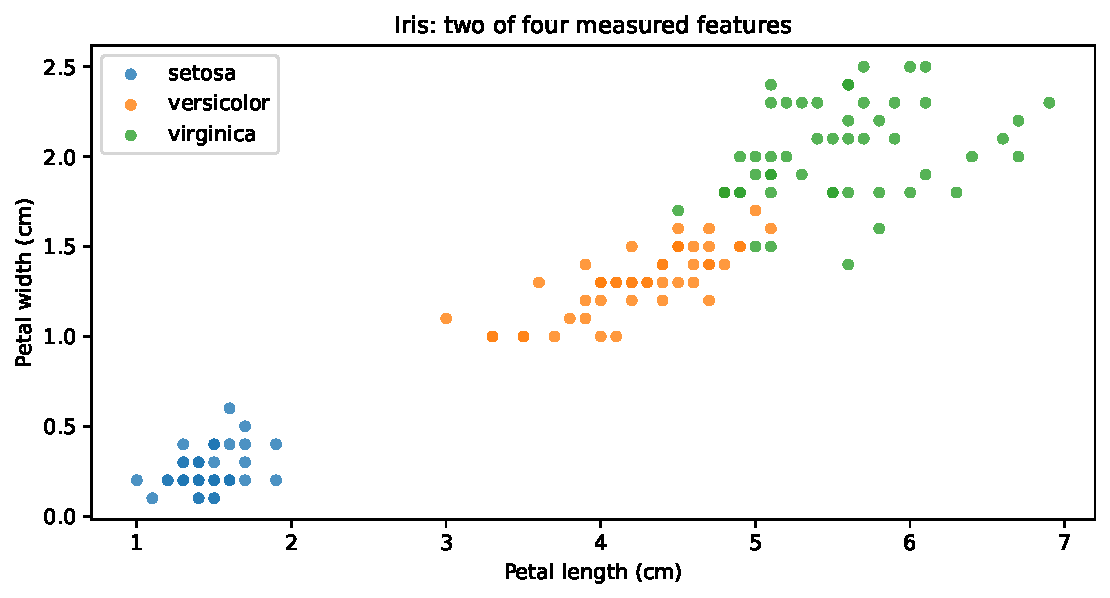
\includegraphics[width=0.83\linewidth]{figures/ch02_iris_scatter.pdf}\caption{鸢尾花两个尺寸的散点图。横纵坐标仅显示四项输入中的两项，不代表已经完成全特征分类。}\label{fig:iris-data}\end{figure}

\textbf{直方图}把一个变量的取值范围分为若干区间，统计各区间记录数，用于观察分布是否集中、偏斜或存在多个峰。画图时应标字段、单位和样本范围，不能只写 \texttt{x}、\texttt{y} 却让读者猜其含义。

\subsection{用分位数和散点图寻找值得追问的记录}
平均值容易受到极端记录影响，中位数表示排序后的中间位置，分位数描述分布的不同部分。四分位距是第75百分位与第25百分位之差，常用于概括中间一半数据的跨度。它们是描述工具，不是自动清洗规则。

例如某个长度列大多数记录在1到10厘米之间，却有一条为500。至少存在三种解释：对象确实很大、该行使用毫米、录入发生错误。只凭“离均值很远”不能确定是哪一种。应回到单位、原始记录和其他相关字段，再决定保留、转换、标记或排除。自动删除极端记录可能恰好删除最值得研究的对象。

相关系数描述两个变量的线性共同变化。两个变量即使相关系数接近零，也可能存在弯曲关系。例如对对称分布的$x$，$y=x^2$可能没有线性相关，却完全由$x$确定。散点图能够补充单个汇总数字看不到的形状。后面线性模型的残差图也采用相同思路：先看模式，再考虑是否需要变换特征或更换模型。

\subsection{缺失和质量字段也有分布}
缺失不是纯粹的软件问题。弱信号可能更难测到某个波段，极端实验条件可能更容易失败。若只保留全部测量齐全的样本，最终研究对象的范围可能发生改变。应记录每一步筛选前后的样本数量，并比较保留与排除记录已有字段的分布。

这不要求初学者立刻掌握复杂的缺失机制模型，但必须学会提出问题：缺失是否与类别、信号强弱或设备条件有关？只有在了解这些关系后，才知道均值填补和删行分别可能造成什么影响。第16章会把这种检查与模型的适用范围联系起来。

\section{缺失值处理与类别编码}
\subsection{缺失不是数值零}
\textbf{缺失值}表示某项记录没有可用值，可能因为未测量、记录丢失或质量不合格。在Pandas中，数值缺失常以 \texttt{NaN} 表示。零是一个具体数值，不能未经解释就代替缺失。原始葡萄酒数据没有缺失；本章Notebook人工遮去少量值，只是为了演示处理步骤，并保留未改动的原表。

\textbf{填补（imputation）}按规定规则为缺失位置提供用于后续计算的替代值。假设训练列为1、缺失、3、8，用已有值的中位数3填补，就得到1、3、3、8。这个3不是恢复出的真实测量，只是一个处理规则的结果。规则所需的中位数从训练数据确定，再应用于验证和测试。

下面同时使用\textbf{NumPy}，这是Python的数值数组工具包，程序中通常简写为\texttt{np}。\textbf{数组}是按固定形状排列的一组数，\texttt{np.nan}表示缺失数值，而不是零。示例先人为制造一个缺失值，用来核对填补步骤，不代表原始葡萄酒数据已有缺失。

\begin{lstlisting}[caption={先手算，再用软件核对中位数填补}]
import numpy as np
from sklearn.impute import SimpleImputer
values = np.array([[1.0], [np.nan], [3.0], [8.0]])
imputer = SimpleImputer(strategy="median")
print(imputer.fit_transform(values).ravel())
print(imputer.statistics_)  # learned replacement: 3
\end{lstlisting}

\subsection{输入类别的独热编码}
假设另一个人工测量表记录仪器类型A、B、C，它们没有数值大小。可以把仪器类型改写为三列：A对应 $(1,0,0)$，B对应 $(0,1,0)$，C对应 $(0,0,1)$。这种表示称为\textbf{独热编码（one-hot encoding）}，每列表示是否属于某类别。它避免把A、B、C直接写成0、1、2后引入并不存在的等间距关系。

这里处理的是\textbf{输入中的类别型特征}，与目标类别用0、1、2保存是不同问题。编码规则也要保存，以便新数据使用相同列顺序。遇到训练时没有出现的仪器类型，需要明确处理办法，而不是临时改动输入列数。

\subsection{填补会改变分布，缺失指示可以保留部分信息}
假设一列四个可用训练值为0、2、4、6，另有四个缺失。用均值3填补后，新增的四个数都落在中心，样本的离散程度变小了。模型看见的表比原始测量更集中，但这并不表示实验精度提高。这是填补规则引入的结构。

可以另外增加一个“原来是否缺失”的二值字段，让模型知道哪些数来自测量、哪些来自填补。这种缺失指示并不一定改善预测，也不能修复偏差，但它避免把估计值与真实测量完全混为一谈。使用时应检查部署数据是否具有类似缺失机制，否则模型可能学到一条只适用于旧设备的数据获取规则。

\subsection{训练中没有见过的类别}
训练只有仪器A和B，应用中出现C时，编码器应按预先规定的策略处理。直接临时增加一列会改变后续模型输入维数；把C强行改成A又会伪造含义。可以使用允许未知类别的编码器、专门的其他类别，或拒绝给出预测并要求补充标定。采取哪一种策略取决于任务，而不是统一越宽松越好。

下面的编码器把已知类别学成固定列，并让未知类别在这些列上为零。零向量仅表示“这些已知指示列都不成立”，不表示新仪器与旧仪器行为相同。后面的线性模型还会叠加截距，所以未知类别仍可能产生一个数值预测，但这个数值的可靠性需要单独检查。
\begin{lstlisting}
from sklearn.preprocessing import OneHotEncoder
encoder = OneHotEncoder(handle_unknown="ignore", sparse_output=False)
encoded_train = encoder.fit_transform([["A"], ["B"], ["A"]])
encoded_new = encoder.transform([["C"]])
print(encoder.categories_, encoded_new)
\end{lstlisting}

\section{特征尺度、标准化与处理流程}
\label{sec:standardization}
\subsection{标准化究竟改变什么}
\textbf{尺度}指变量数值变化的量级。葡萄酒的某些指标取值接近个位数，另一些可达到数百甚至上千。如果算法依据数值差计算距离，较大的尺度可能支配结果。长度由米换成毫米也会放大数字，却没有改变对象本身，这提示我们要区分测量含义和数值表示。

\textbf{标准化（standardization）}在本书指用训练均值 $\mu$ 减去中心，再除以训练标准差 $s$：
\[
z=\frac{x-\mu}{s}.
\]
$z$表示某个值高于或低于训练均值多少个标准差。对训练值1、2、3，采用分母为3的方差约定，$\mu=2$，$s=\sqrt{2/3}\approx0.8165$，变换后约为 $-1.225,0,1.225$。一个后来出现的值4应使用同一个均值和标准差，得到约2.449，不能单独对这个新值重新计算中心和尺度。\texttt{StandardScaler}使用的方差分母为训练记录数，其零方差列另有安全处理\textsuperscript{[31]}。

\fig{ch02_wine_scales.pdf}{葡萄酒部分测量字段在原始与标准化表示中的尺度。标准化使单位尺度可比较，不保证任意分类方法的效果都会提高。}

\subsection{fit与transform分别完成什么}
\begin{lstlisting}[caption={把学习尺度和应用尺度分成两步}]
from sklearn.preprocessing import StandardScaler
scaler = StandardScaler()
scaler.fit(X_dev)
X_dev_scaled = scaler.transform(X_dev)
# Do not fit the scaler again on the held-out records.
X_hold_scaled = scaler.transform(X_hold)
print(scaler.mean_[:3], scaler.scale_[:3])
\end{lstlisting}
对这个变换器，\texttt{fit}只从输入计算均值和尺度，没有学习类别；\texttt{transform}按已保存的规则改变数值。\texttt{fit\_transform}把两步合并，适用于学习规则的训练数据，不应在测试数据上重新调用来得到另一套尺度。

\textbf{流水线（Pipeline）}把若干处理步骤按顺序连起来。例如“填补缺失—标准化—分类模型”是一个整体：训练时前面的步骤学习处理规则，后面的模型学习预测规则；预测时所有步骤应用已经保存的规则。第4章将用它在每次验证中重新建立训练流程。先理解这里的手动两步，再理解流水线为什么能减少漏做或错用步骤的风险。

\textbf{归一化}在不同资料中含义不完全一致，有时指缩放到固定区间，有时指把整个样本向量缩放为固定长度。本书不把它作为所有尺度处理的统称；报告中写明实际公式或所用变换器。标准化也不能修复错误标签或补全测量信息，它只改变数值表示。

\subsection{尺度变换怎样改变距离和参数含义}
考虑两维输入：长度以米计，质量以千克计。两点的欧氏距离平方写成$(\Delta x_1)^2+(\Delta x_2)^2$，把长度换成毫米后，第一项放大一百万倍。物理对象没有改变，但默认距离的相对权重改变了。标准化相当于先给每个方向规定一个比较尺度，再计算距离，因此需要与“相似”的含义一起考虑。

对线性预测$\hat y=b+wz$，若$z=(x-\mu)/s$，则
\[
\hat y=\left(b-\frac{w\mu}{s}\right)+\frac{w}{s}x.
\]
所以标准化坐标中的系数不是原始单位下的斜率。可以通过这个代换把参数还原，不必把变换后的模型看成无法解释的对象。若有多个特征，对每列分别换算并把所有截距修正加总即可。这个关系会在第5章系数解释中使用。

标准化不能保证分布变成正态分布。一个明显偏斜、有两个峰或含极端值的分布，减均值除标准差以后仍可能保留相同形状。它也不等于把所有值限制在$[0,1]$，验证记录完全可以超过训练均值很多个标准差。\textbf{处理公式决定它改变什么，名称不能代替公式。}

\subsection{一次可以复核的数据准备实验}
随书实验在葡萄酒训练数据中，人工遮去8个酒精测量值，并保存原位置清单。它先用训练中位数填补，再用训练均值和标准差缩放，最后把同一流程应用到验证数据。实验没有修改原始公开数据文件，也没有宣称这些缺失来自真实采样。

训练变换后的各列均值接近零，这是标准化的定义结果；验证列均值通常不等于零，这是合理现象，因为验证记录与训练记录不同。不要为了让验证均值也恰好为零，再在验证数据上拟合一个新的缩放器。检查时应核对处理规则是否一致，而不是要求所有数据都出现同样的统计数字。

\subsection{怎样组织不同类型字段的处理}
实际表格可能同时含有数值字段与类别字段。数值字段可以依次填补、缩放，类别字段可以填补后独热编码。\texttt{ColumnTransformer}按列把这些不同流程并行组织起来；\texttt{Pipeline}再把合并后的特征送给模型。两者不是额外的机器学习算法，而是保存数据处理顺序和字段角色的工具。

初次练习时可以手动完成一列变换，等每一步含义清楚后再组合。最终提交应保存字段顺序、已学习的中位数或类别表、缩放参数及模型。只保存最后一组模型系数，往往不足以在新数据上重现同样的预测。

\chapterpractice{用葡萄酒数据完成读取、保存CSV、重新读入和字段角色检查；手算本章的中位数填补和标准化例子，再用代码核对；在开发数据上计算字段统计量和绘图；说明保留数据为什么只应用处理规则。算法性能比较留到第4章以后。}
\chapterexercise
\begin{enumerate}
\item 葡萄酒数据中，一行表示什么？13项输入与类别列各承担什么角色？为什么这不是品质评分任务？
\item \texttt{X[["alcohol"]]}与\texttt{X.iloc[[0]]}在形状和含义上有什么不同？
\item 对训练值2、4、6，采用分母为3的方差进行标准化；再将新值8按训练规则变换。写出各步结果。
\item 缺失值与零有什么不同？中位数填补能否恢复没有测到的真实数值？
\item 为什么在测试部分重新调用\texttt{fit\_transform}可能改变模型实际看到的特征含义？
\end{enumerate}

\section*{深化练习与方法检验}
本组题强调解释、计算与验证；D编号在本章内独立计数。计算题应写出所用定义和中间步骤，实验题保留实际输出，包括不支持预期的结果。
\begin{enumerate}[label=D\arabic*.]
\item 主表有对象A、B两行，辅助表中A出现三次、B出现一次。按对象编号合并后有几行？怎样检验原本期望的一对一关系，为什么直接在合并后随机拆行可能产生问题？
\item 对训练列 $(1,3,5)$ 用分母为3的方差标准化，并把新值7变换到同一坐标。再说明：把训练值与新值合并后重新计算均值，得到的是不是同一个预测流程？
\item 一个输入字段缺失时，仪器往往处于低信噪比状态。只用中位数填补可能遗漏什么信息？设计一种保留“是否缺失”的表示，并说明它可能在哪种部署变化下失效。
\item 长度从米改为毫米后，原始欧氏距离、标准化后的距离、按单特征顺序划分的训练分组分别可能怎样变化？解释为什么“单位改变没有物理变化”不等于所有算法自动保持数值结果。
\end{enumerate}
